\documentclass[12pt,a4paper]{article}
\usepackage[utf8]{vietnam}
\usepackage{amsmath,amssymb}
\usepackage{geometry}
\geometry{top=1.5cm,bottom=1.2cm,left=1.4cm,right=1.4cm,headheight=28pt,headsep=12pt,footskip=18pt}
\usepackage{tikz}
\usepackage{xcolor}
\usepackage{enumerate}
\usepackage{graphicx}
\usepackage[version=4]{mhchem}
\usepackage{fancyhdr}
\usepackage{ex_test}

\renewcommand{\baselinestretch}{1.0}
\setlength{\parskip}{1pt}

\definecolor{hfRed}{RGB}{211,47,47}
\definecolor{hfGreen}{RGB}{139,195,144}

\pagestyle{fancy}
\fancyhf{}
\fancyhead[L]{\small\itshape\color{hfRed} Tài liệu lưu hành nội bộ}
\fancyhead[R]{\small\itshape\color{hfRed} Thầy \textbf{TRẦN VĂN THẠNH} - 0777.470.803}
\renewcommand{\headrulewidth}{0.8pt}
\renewcommand{\headrule}{\hbox to\headwidth{\color{hfGreen}\leaders\hrule height \headrulewidth\hfill}}

\fancyfoot[L]{\small\itshape\color{hfRed} CS1: 6/15 Nguyễn Hoàng, P. Kim Long, TP Huế \quad|\quad CS2: 24 Đặng Thái Thân, TP Huế}
\fancyfoot[R]{\small\bfseries\color{hfRed} Trang \thepage}
\renewcommand{\footrulewidth}{0.8pt}
\renewcommand{\footrule}{\hbox to\headwidth{\color{hfGreen}\leaders\hrule height \footrulewidth\hfill}}

\fancypagestyle{firstpage}{
  \fancyhf{}
  \renewcommand{\headrulewidth}{0pt}
  \fancyfoot[L]{\small\itshape\color{hfRed} CS1: 6/15 Nguyễn Hoàng, P. Kim Long, TP Huế \quad|\quad CS2: 24 Đặng Thái Thân, TP Huế}
  \fancyfoot[R]{\small\bfseries\color{hfRed} Trang \thepage}
  \renewcommand{\footrulewidth}{0.8pt}
  \renewcommand{\footrule}{\hbox to\headwidth{\color{hfGreen}\leaders\hrule height \footrulewidth\hfill}}
}

\begin{document}
\thispagestyle{firstpage}

\noindent
\begin{minipage}[t]{0.45\textwidth}
	\centering\fontsize{10pt}{12pt}\selectfont
	\textbf{SỞ GD\&ĐT THÀNH PHỐ HUẾ}\\
	\textbf{TRƯỜNG THPT PHONG ĐIỀN}\\
	\textbf{ĐỀ CHÍNH THỨC}\\
	\textit{(Đề thi có 04 trang)}
\end{minipage}\hfill
\begin{minipage}[t]{0.53\textwidth}
	\centering\small
	\textbf{KIỂM TRA GIỮA HỌC KỲ I -- NĂM HỌC 2025 - 2026}\\
	\textbf{MÔN: HOÁ HỌC 11 CTST}\\
	\textit{Thời gian làm bài: 45 phút (không kể thời gian phát đề)}\\
	\fbox{\textbf{MÃ ĐỀ: 504}}
\end{minipage}

\smallskip
\noindent\hrulefill
\smallskip

\noindent\textbf{Họ, tên thí sinh:} \dotfill\ \textbf{Lớp:} \dotfill\ \textbf{Số báo danh:} \dotfill

\smallskip
\noindent\textit{(Cho biết nguyên tử khối: H = 1; C = 12; N = 14; O = 16; Na = 23; S = 32; Cl = 35,5; Fe = 56).}
\smallskip

\noindent
\textbf{PHẦN I. Câu trắc nghiệm nhiều phương án lựa chọn.}\\
\textit{Thí sinh trả lời từ câu 1 đến câu 12. Mỗi câu hỏi thí sinh chỉ chọn một phương án.}

\Opensolutionfile{ans}[ans-hoa11-ma504hs]

\begin{ex}
Cân bằng hóa học là một cân bằng
\choice
{Đứng yên}
{Tĩnh}
{Cố định}
{Động}
\loigiai{}
\end{ex}

\begin{ex}
Trong thí nghiệm đốt cháy sulfur (S) trong không khí, hiện tượng nào sau đây có thể được quan sát?
\choice
{Sulfur cháy với ngọn lửa màu đỏ và sinh ra khói trắng}
{Sulfur cháy với ngọn lửa màu xanh và sinh ra khí không màu, mùi hắc}
{Sulfur cháy với ngọn lửa màu tím và sinh ra khí không mùi}
{Sulfur cháy với ngọn lửa màu vàng nhạt và sinh ra khí có mùi ngọt}
\loigiai{}
\end{ex}

\begin{ex}
Nạp đầy khí amoniac vào bình thuỷ tinh trong suốt, đậy bình $\ce{NH3}$ bằng nút cao su có ống thuỷ tinh vuốt nhọn xuyên qua. Nhúng đầu ống thuỷ tinh vào một chậu thuỷ tinh chứa nước có pha thêm dung dịch phenolphthalein. Một lát sau, nước trong chậu phun vào bình thành những tia có màu hồng. Thí nghiệm này chứng tỏ được:
\choice
{$\ce{NH3}$ là chất khí.}
{$\ce{NH3}$ tan nhiều trong nước.}
{$\ce{NH3}$ có mùi khai.}
{$\ce{NH3}$ có tính bazơ và tan nhiều trong nước.}
\loigiai{}
\end{ex}

\begin{ex}
Nitrogen monoxide được tạo thành khi mưa dông kèm theo sấm sét do phản ứng giữa nitrogen và oxygen trong không khí được gọi là
\choice
{$\ce{NO_x}$ nhiên liệu.}
{$\ce{NO_x}$ tức thời.}
{$\ce{NO_x}$ tự nhiên.}
{$\ce{NO_x}$ nhiệt.}
\loigiai{}
\end{ex}

\begin{ex}
Cho các nhận định sau về cấu tạo phân tử nitric acid:\\
(a) Liên kết $\ce{O - H}$ phân cực về oxygen.\\
(b) Nguyên tử N có số oxi hóa là $+5$.\\
(c) Nguyên tử N có hóa trị bằng IV.\\
(d) Liên kết cho -- nhận $\ce{N -> O}$ kém bền.\\
Số nhận định đúng là
\choice
{4.}
{1.}
{2.}
{3.}
\loigiai{}
\end{ex}

\begin{ex}
Đâu là phát biểu của thuyết Bronsted-Lowry?
\choice
{Acid là chất nhận proton, base là chất cho proton}
{Cả acid và base đều là chất nhận proton}
{Acid là chất cho proton, base là chất nhận proton}
{Cả acid và base đều là chất cho proton}
\loigiai{}
\end{ex}

\begin{ex}
Xét cân bằng: $\ce{N2(g) + 3H2(g) <=> 2NH3(g)}$. Biểu thức hằng số cân bằng của phản ứng là:
\choice
{$K = \frac{[\ce{N2}][\ce{H2}]}{[\ce{NH3}]}$}
{$K = \frac{[\ce{NH3}]}{[\ce{N2}][\ce{H2}]}$}
{$K = \frac{[\ce{NH3}]^2}{[\ce{N2}][\ce{H2}]^3}$}
{$K = \frac{[\ce{N2}][\ce{H2}]^3}{[\ce{NH3}]^2}$}
\loigiai{}
\end{ex}

\begin{ex}
Hợp chất nào sau đây của sulfur được sử dụng để khử trùng và tẩy trắng trong công nghiệp?
\choice
{$\ce{SO2}$}
{$\ce{H2SO4}$}
{$\ce{S8}$}
{$\ce{H2S}$}
\loigiai{}
\end{ex}

\begin{ex}
Trong tự nhiên luôn diễn ra các quá trình chuyển hóa nitrogen từ dạng này sang dạng khác theo...
\choice
{Một chu trình tuần hoàn không khép kín}
{Một chu trình tuần hoàn khép kín}
{Một chu trình ngẫu nhiên}
{Một chu trình không tuần hoàn}
\loigiai{}
\end{ex}

\begin{ex}
pH là
\choice
{Chỉ số đánh giá độ acid của một dung dịch}
{Chỉ số đánh giá độ acid hay độ base của một dung dịch}
{Chỉ số đánh giá độ base của một dung dịch}
{Chỉ số đánh giá các chất điện li mạnh}
\loigiai{}
\end{ex}

\begin{ex}
Tính chất nào sau đây là tính chất vật lý của sulfur (S)?
\choice
{Là chất khí không màu}
{Là chất rắn màu vàng, không tan trong nước}
{Tan tốt trong nước}
{Dễ bay hơi ở nhiệt độ thường}
\loigiai{}
\end{ex}

\begin{ex}
Cho các nhận định sau về tính chất hoá học của nitric acid: (1) có tính acid mạnh; (2) có tính acid yếu; (3) có tính oxi hoá mạnh; (4) có tính khử mạnh. Số nhận định đúng là
\choice
{4.}
{1.}
{2.}
{3.}
\loigiai{}
\end{ex}

\Closesolutionfile{ans}

\bigskip
\noindent
\textbf{PHẦN II. Câu trắc nghiệm đúng sai. (2 điểm)}\\
\textit{Trong mỗi ý a), b), c), d) ở mỗi câu, thí sinh chọn đúng hoặc sai. Điểm tối đa của 01 câu hỏi là 1 điểm:}\\
\textit{- Thí sinh chỉ lựa chọn chính xác 01 ý trong 1 câu hỏi được 0,1 điểm.}\\
\textit{- Thí sinh chỉ lựa chọn chính xác 02 ý trong 1 câu hỏi được 0,25 điểm.}\\
\textit{- Thí sinh chỉ lựa chọn chính xác 03 ý trong 1 câu hỏi được 0,5 điểm.}\\
\textit{- Thí sinh chỉ lựa chọn chính xác 04 ý trong 1 câu hỏi được 1 điểm.}

\begin{ex}
Ammonium nitrate được dùng làm phân đạm. Năm 2020, một vụ nổ tại thủ đô Beirut, Lebanon đã cướp đi sinh mạng của hàng trăm người. Nguyên nhân của vụ nổ được do sự phân huỷ 2750 tấn ammonium nitrate trên một tàu hàng bỏ hoang theo phương trình hoá học sau:
\[ \ce{NH4NO3(s) -> N2O(g) + 2H2O(g)} \quad \Delta_r H_{298}^\circ = -36\text{ kJ} \]
\choiceTF
{a) Phản ứng (1) là phản ứng thu nhiệt.}
{b) Dung dịch muối Ammonium nitrate phản ứng với dung dịch base đặc, nóng thoát ra chất khí làm quỳ tím ẩm hoá đỏ.}
{c) Khi bón phân đạm ammonium nitrate nhiều sẽ gây hiện tượng chua đất.}
{d) Nhiệt của vụ nổ trên tương đương với nhiệt toả ra 1062 tấn thuốc nổ TNT. (biết 1 kg thuốc nổ TNT phát nổ toả ra $1{,}165 \cdot 10^6\text{ J}$).}
\loigiai{}
\end{ex}

\begin{ex}
Một học sinh làm thí nghiệm xác định pH của đất như sau: lấy một lượng đất cho vào nước rồi lọc lấy phần dung dịch. Dùng máy đo pH đo được $\text{pH} = 4{,}69$.
\choiceTF
{a) Môi trường của dung dịch là acid.}
{b) Loại đất trên được gọi là đất chua. Để giảm độ chua cho đất có thể bón vôi.}
{c) Dung dịch trong cốc có $[\ce{OH-}] > [\ce{H+}]$ vì $\text{pOH} > \text{pH}$.}
{d) Nồng độ $[\ce{H+}]$ trong cốc lớn hơn 0,001.}
\loigiai{}
\end{ex}

\bigskip
\noindent
\textbf{PHẦN III: Câu trắc nghiệm yêu cầu trả lời ngắn. (2 điểm)}\\
\textit{Thí sinh trả lời từ câu 1 đến câu 4.}

\begin{ex}
Tổng số liên kết $\sigma$ và số liên kết $\pi$ trong phân tử nitrogen là bao nhiêu?
\shortans{}
\loigiai{}
\end{ex}

\begin{ex}
Để giảm thải lượng khí thải $\ce{SO2}$ ra môi trường, trong các biện pháp sau:\\
(1) Sử dụng nguồn nhiên liệu sinh học thân thiện với môi trường như hydrogen, ethanol.\\
(2) Sử dụng nguồn năng lượng hóa thạch.\\
(3) Sử dụng nguồn năng lượng tái tạo như năng lượng mặt trời, năng lượng gió, mưa, sóng biển, thủy triều, địa nhiệt.\\
(4) Xử lý khí thải công nghiệp trước khi thải ra môi trường.\\
Cần thực hiện biện pháp nào trong số các biện pháp trên?
\shortans{}
\loigiai{}
\end{ex}

\begin{ex}
Dịch vị dạ dày của con người có chứa hydrochloric acid ($\ce{HCl}$), với pH dao động trong khoảng 2-4. Những người bị mắc bệnh viêm loét dạ dày, tá tràng thường có $\text{pH} < 2$. Nabica (có thành phần chính là $\ce{NaHCO3}$) là một loại thuốc được dùng để trung hoà bớt lượng acid trong dạ dày của những bệnh nhân có pH trong dạ dày thấp và thường được uống trước bữa ăn. Giả sử một bệnh nhân bị đau dạ dày đã uống $0{,}504\text{ gam}$ bột $\ce{NaHCO3}$. Hãy tính số mol $\ce{HCl}$ đã được trung hòa.
\shortans{}
\loigiai{}
\end{ex}

\begin{ex}
Cho các phát biểu sau:\\
(a) Trong không khí, Nitrogen chiếm khoảng 78\% về thể tích.\\
(b) Trong bầu khí quyển, khi có sấm chớp, khí nitrogen tạo các nitrogen oxide, là một nguyên nhân làm cho nước mưa có tính acid.\\
(c) Trong phản ứng giữa $\ce{N2}$ và $\ce{H2}$ thì $\ce{N2}$ là chất khử.\\
(d) Phần lớn Nitrogen được sử dụng để tổng hợp $\ce{NH3}$, từ đó sản xuất nitric acid, phân bón.\\
Số phát biểu đúng là bao nhiêu?
\shortans{}
\loigiai{}
\end{ex}

\bigskip
\noindent
\textbf{PHẦN IV: Tự luận (3 điểm)}

\begin{ex}
\textbf{(0,5 điểm)} Giải thích vì sao khi mở nắp chai nước có gas, dung dịch bị sủi bọt mạnh, sau đó giảm dần.
\loigiai{}
\vspace*{3cm}
\end{ex}

\begin{ex}
\textbf{(0,5 điểm)} Một nhà máy thải ra $1000\text{ m}^3$ khí chứa $0{,}05\%$ thể tích $\ce{SO2}$ mỗi ngày. Tính khối lượng $\ce{SO2}$ (tính bằng kg) thải ra trong ngày (ở đktc).
\loigiai{}
\vspace*{3cm}
\end{ex}

\begin{ex}
\textbf{(0,5 điểm)} Giải thích vì sao khí nitrogen ($\ce{N2}$) trơ về mặt hóa học ở điều kiện thường.
\loigiai{}
\vspace*{3cm}
\end{ex}

\begin{ex}
\textbf{(1,0 điểm)} Một khu ruộng rau có lớp đất mặt dày $10\text{ cm}$, khối lượng riêng $1{,}2\text{ g/cm}^3$, có khả năng trao đổi cation -- Cation Exchange Capacity (CEC) là $5\text{ cmol}_{\text{c}}\text{/kg}$ và tỉ lệ bão hòa bazo là $10\%$. Trong mùa mưa, tổng lượng mưa là $400\text{ mm}$, trung bình $\text{pH} = 2{,}8$ (do ô nhiễm khí $\ce{NO2}$ và $\ce{SO2}$ trong không khí). Biết: $1\text{ mm}$ mưa trên $1\text{ ha} = 10\text{ m}^3\text{ nước} = 10^4\text{ L}$; $[\ce{H+}] = 10^{-\text{pH}}\text{ mol/L}$; $1\text{ mol }\ce{H+}$ trung hòa $1\text{ mol}$ điện tích bazo ($\text{mol}_{\text{c}}$).\\
Câu hỏi:
\begin{enumerate}
	\item Tính số mol $\ce{H+}$ do lượng mưa này mang xuống $1\text{ ha}$ đất (làm tròn đến hàng chục mol).
	\item Tính lượng mol bazo sẵn có trong lớp đất ($10\text{ cm}$) của $1\text{ ha}$.
	\item So sánh hai giá trị trên và kết luận xem mưa acid có thể gây hạ pH đất hay không. Giải thích ngắn gọn vì sao pH đất giảm lại có thể gây hại cho cây trồng.
\end{enumerate}
\loigiai{}
\vspace*{6cm}
\end{ex}

\begin{ex}
\textbf{(0,5 điểm)} Ở trạng thái bình thường, dịch vị dạ dày thường có nồng độ $[\ce{H+}]$ là $2 \cdot 10^{-4}\text{ M}$. Khi tiến hành tiêu hóa, thức ăn đi vào dạ dày làm giải phóng acid $\ce{HCl}$ và dịch vị dạ dày cũng vì vậy mà có giá trị thay đổi, khi này nồng độ ion $[\ce{H+}]$ là $4 \cdot 10^{-2}\text{ M}$.\\
Tính giá trị pH của dạ dày ở trạng thái bình thường và khi dạ dày tiêu hóa thức ăn.
\begin{center}
	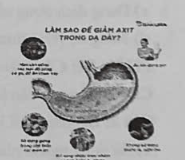
\includegraphics[width=0.35\textwidth]{images_crop/de504_da_day.png}
\end{center}
\loigiai{}
\vspace*{3.5cm}
\end{ex}

\begin{center}
\textbf{--------- HẾT ---------}\\
\textit{(Học sinh không sử dụng tài liệu và bảng tuần hoàn hoá học)}
\end{center}

\end{document}
